\clearpage
\appendix
\phantomsection
\addcontentsline{toc}{section}{Appendix A: Additional Figures}
\section*{Appendix A: Additional Figures}
\setcounter{figure}{0}
\renewcommand{\thefigure}{A\arabic{figure}}
\setcounter{table}{0}
\renewcommand{\thetable}{A\arabic{table}}

\begin{figure}[htbp]
  \centering
  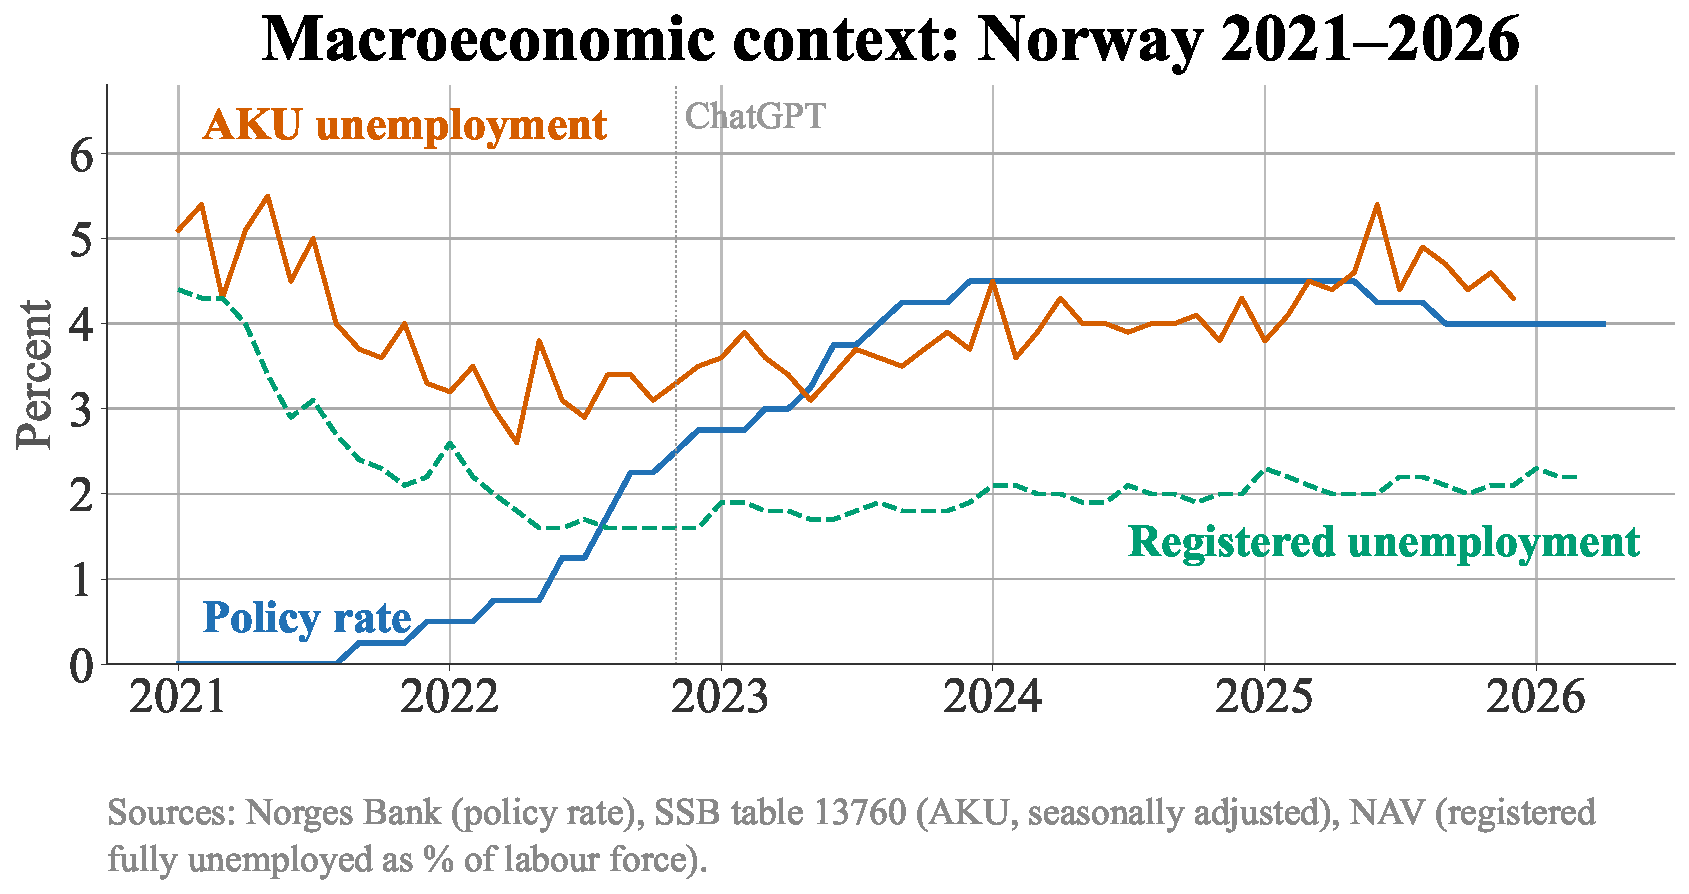
\includegraphics[width=0.8\textwidth]{../analysis/output/figures/figureA0a_macro_context.pdf}
  \caption{Macroeconomic context: Norges Bank policy rate and registered unemployment rate, 2015--2025.}
  \label{fig:macro_context}
\end{figure}

\begin{figure}[htbp]
  \centering
  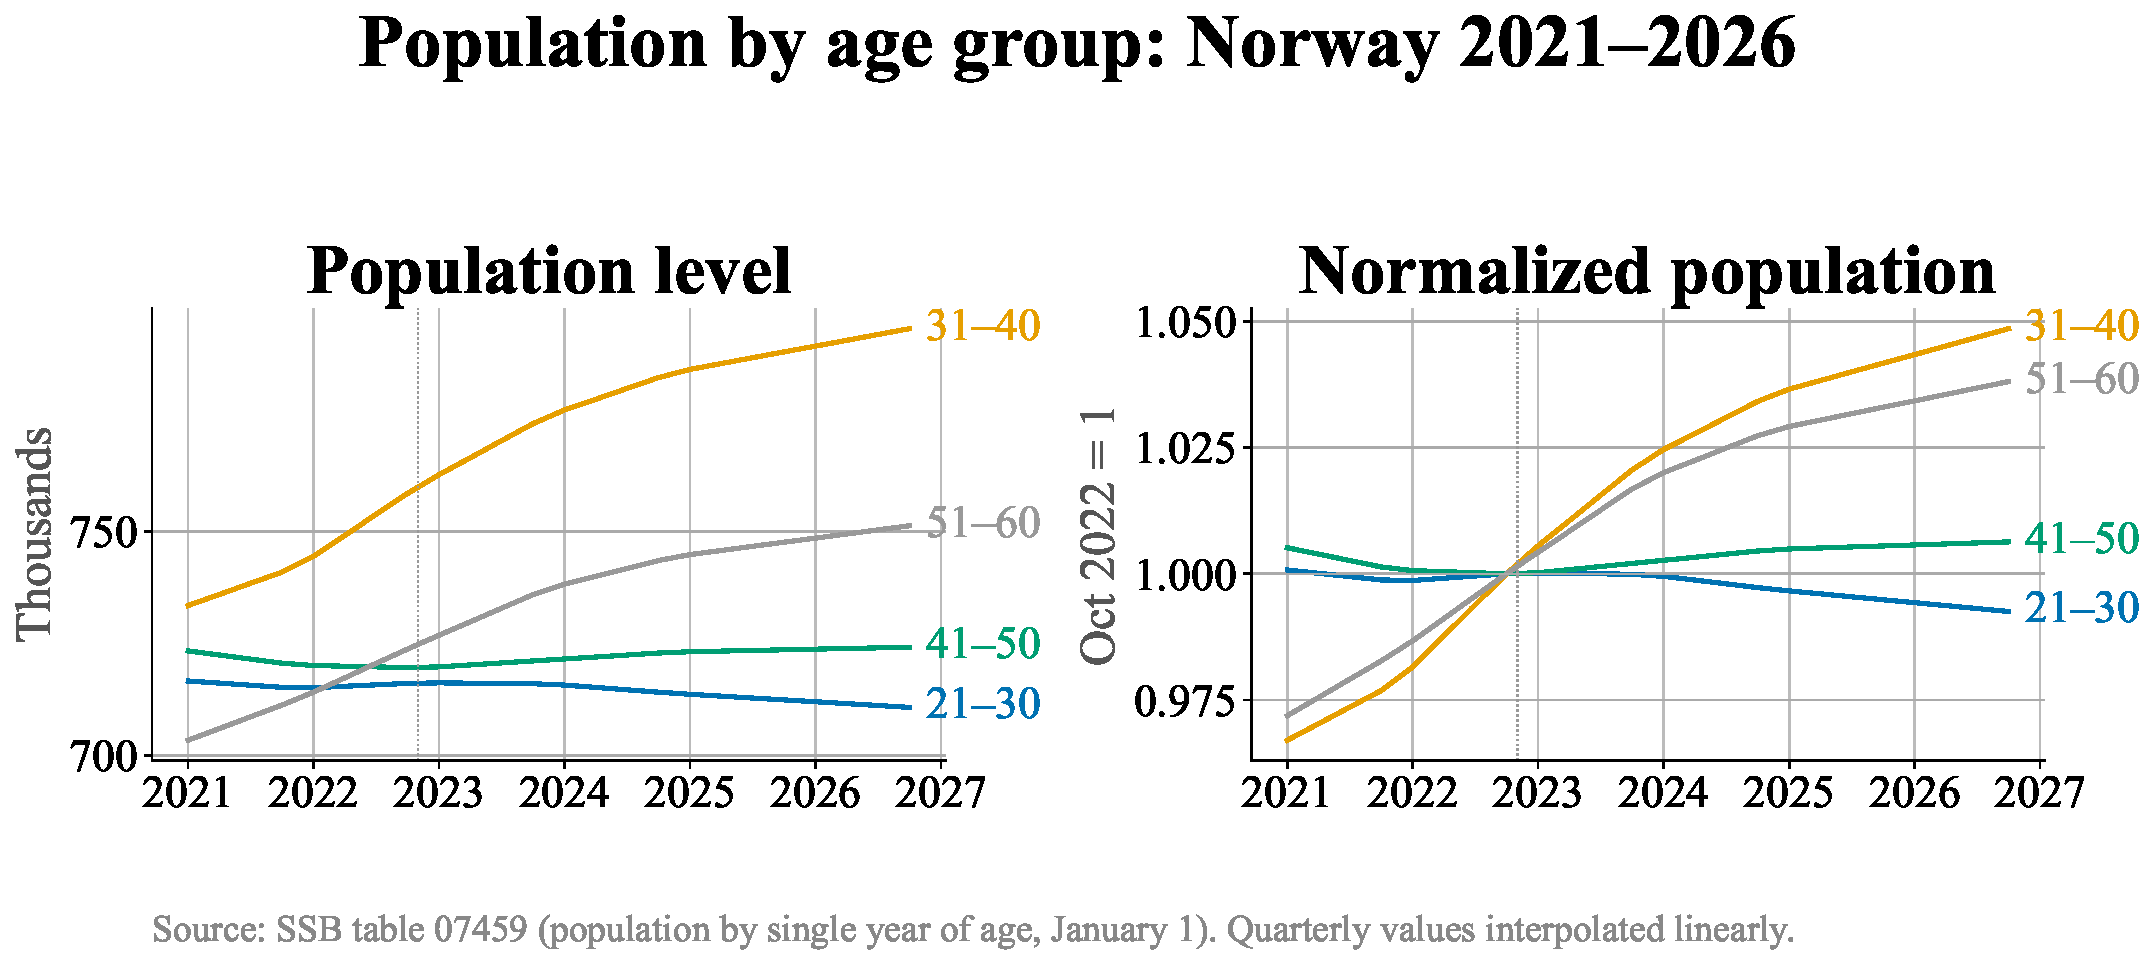
\includegraphics[width=0.8\textwidth]{../analysis/output/figures/figureA0b_cohort_sizes.pdf}
  \caption{Resident population by decade age group, 2015--2025.}
  \label{fig:cohort_sizes}
\end{figure}

\begin{figure}[htbp]
  \centering
  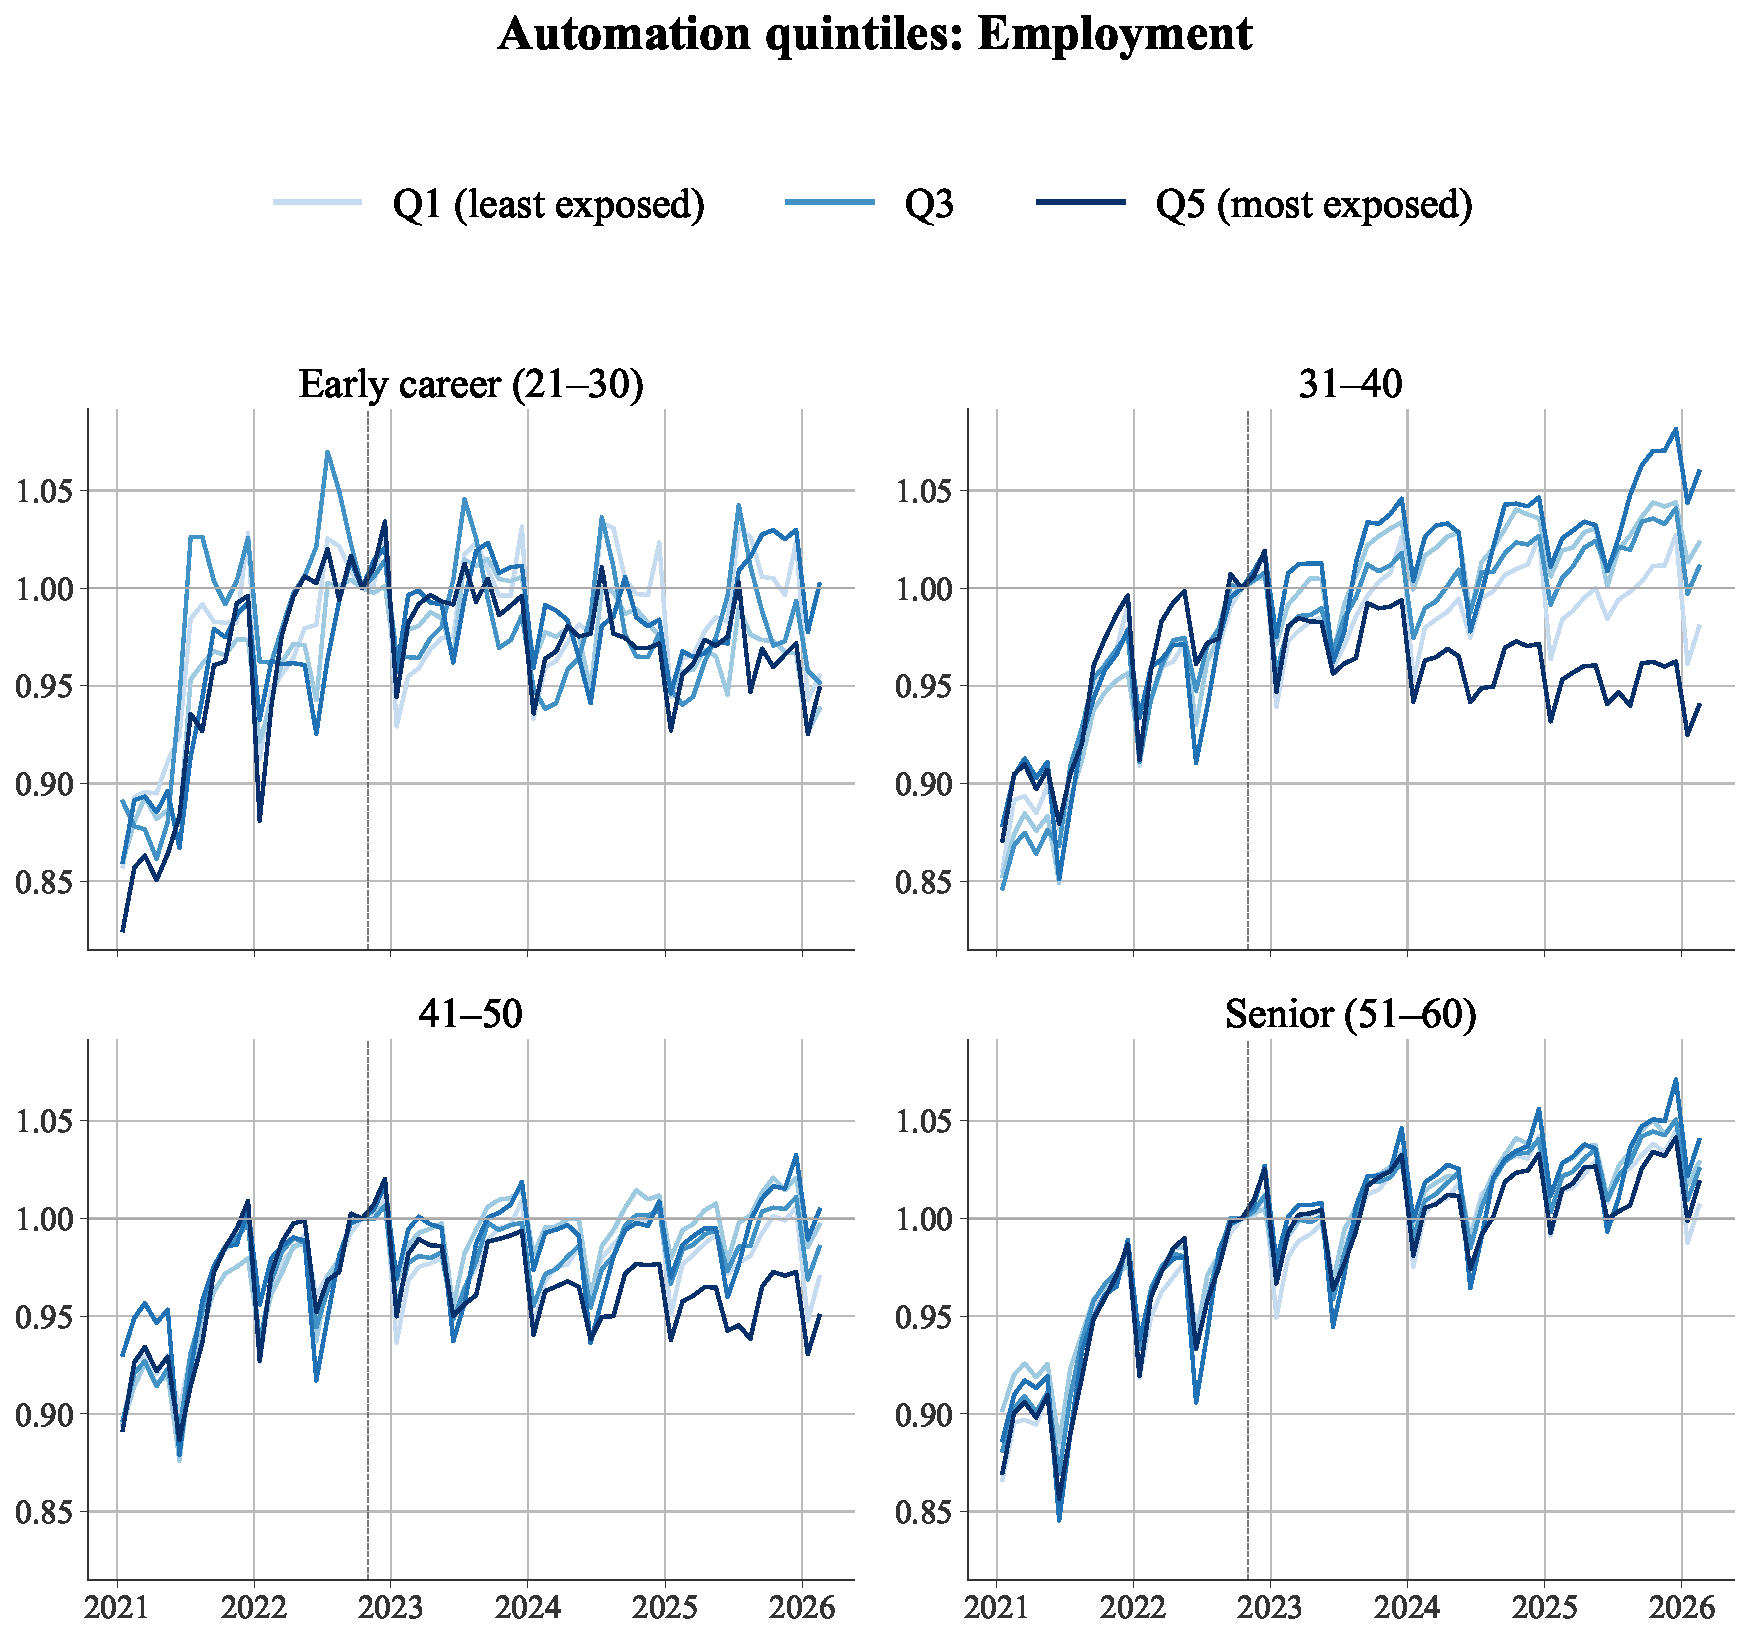
\includegraphics[width=\textwidth]{../analysis/output/figures/figure5b_age_by_quintile_handa.pdf}
  \caption{Employment by Handa et al.\ automation-exposure quintile and decade age group, private sector.}
  \label{fig:age_by_quintile_handa_auto}
  \begin{minipage}{\textwidth}\footnotesize\textit{Notes:} Private-sector employment indexed to October 2022 = 1. Occupations are ranked by the Handa et al.\ automation share.\end{minipage}
\end{figure}

\begin{figure}[htbp]
  \centering
  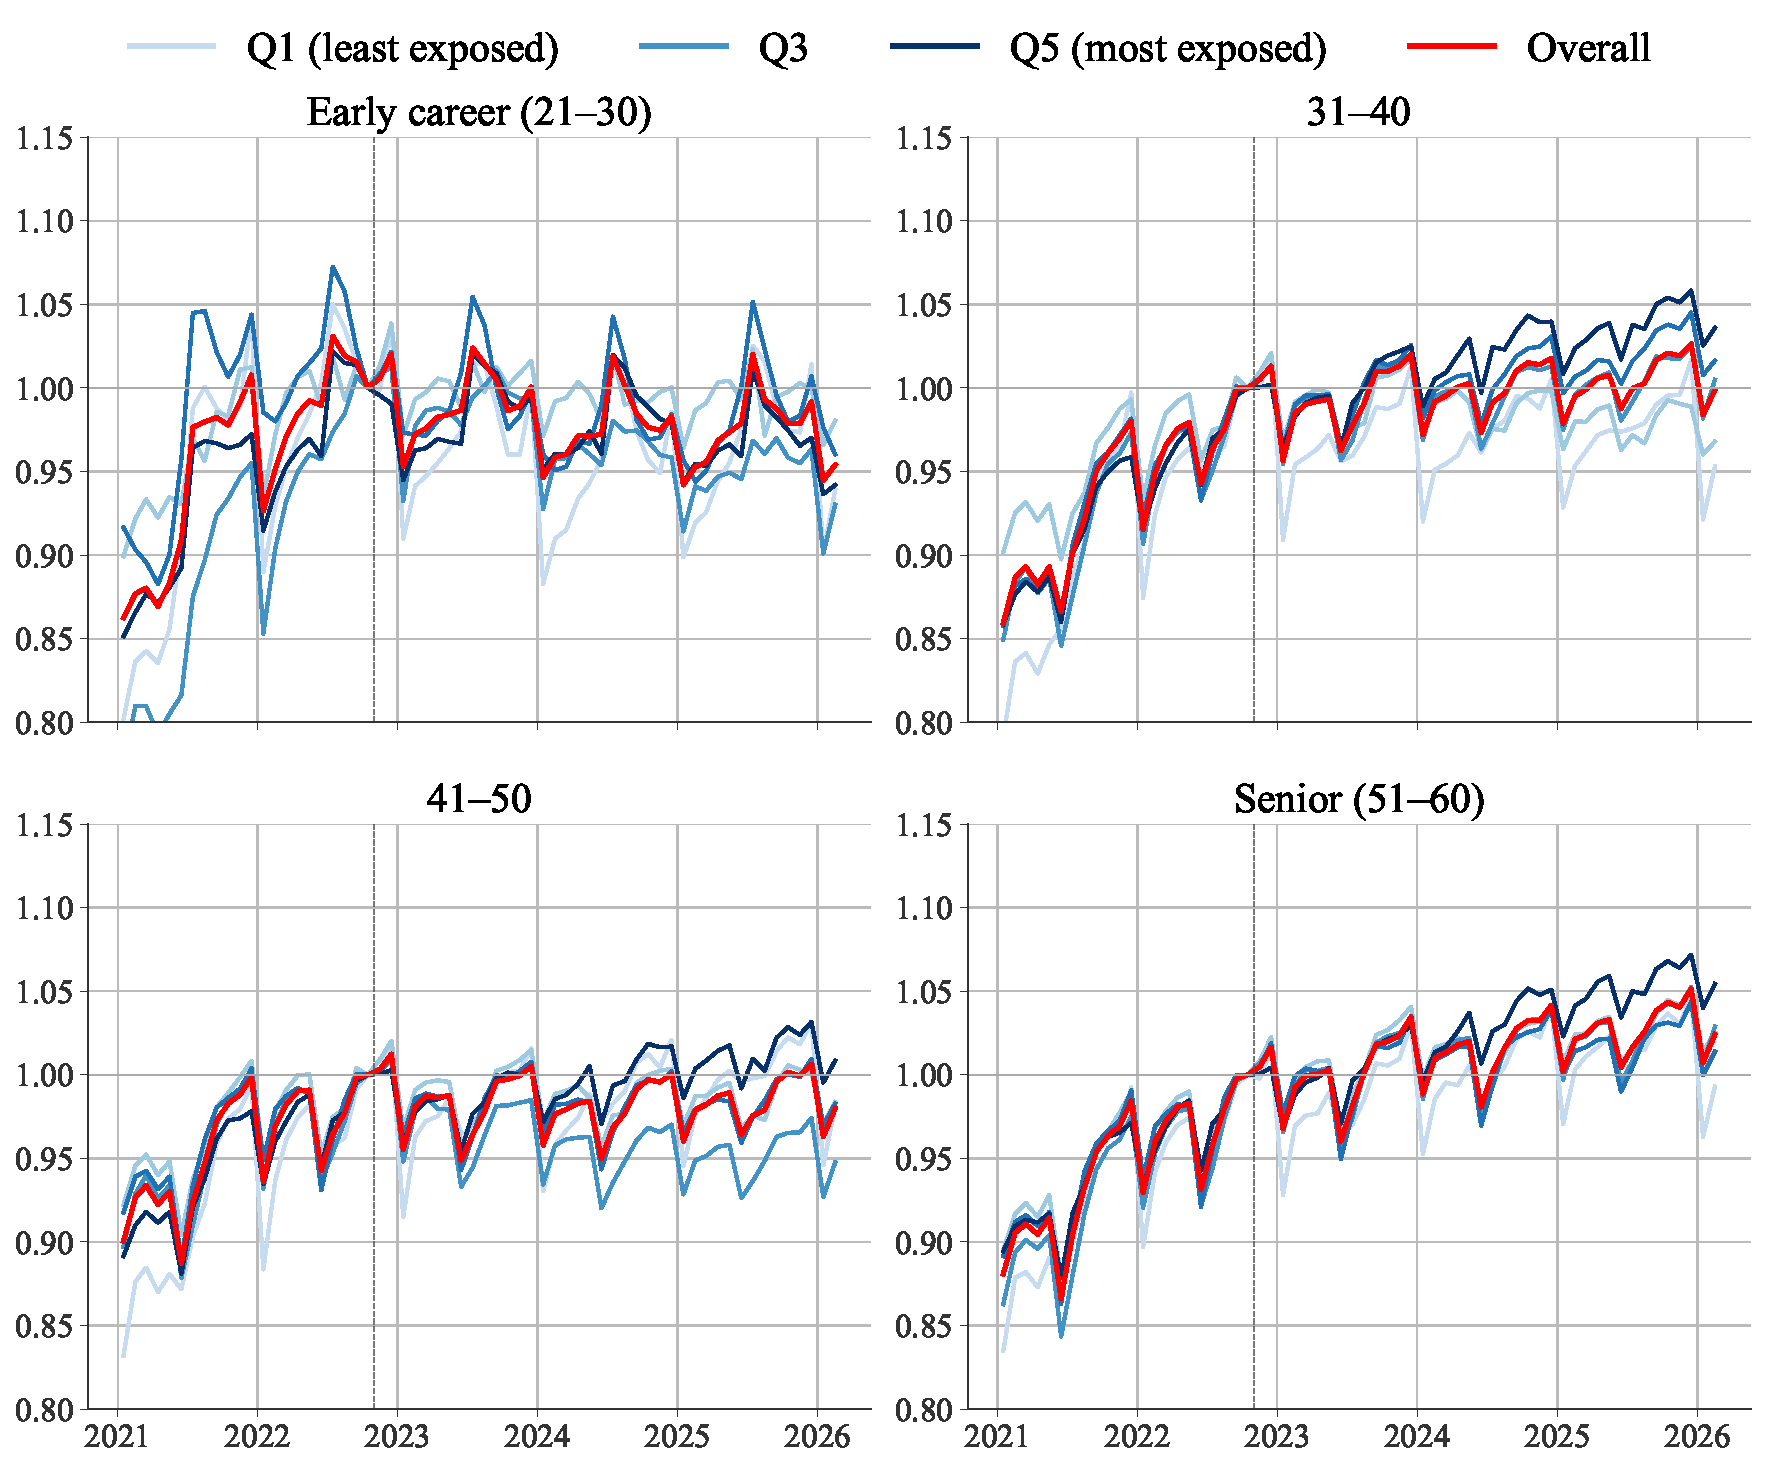
\includegraphics[width=\textwidth]{../analysis/output/figures/figure5c_age_by_quintile_handa.pdf}
  \caption{Employment by Handa et al.\ augmentation-exposure quintile and decade age group, private sector.}
  \label{fig:age_by_quintile_handa_aug}
  \begin{minipage}{\textwidth}\footnotesize\textit{Notes:} Private-sector employment indexed to October 2022 = 1. Occupations are ranked by the Handa et al.\ augmentation share.\end{minipage}
\end{figure}

\begin{figure}[htbp]
  \centering
  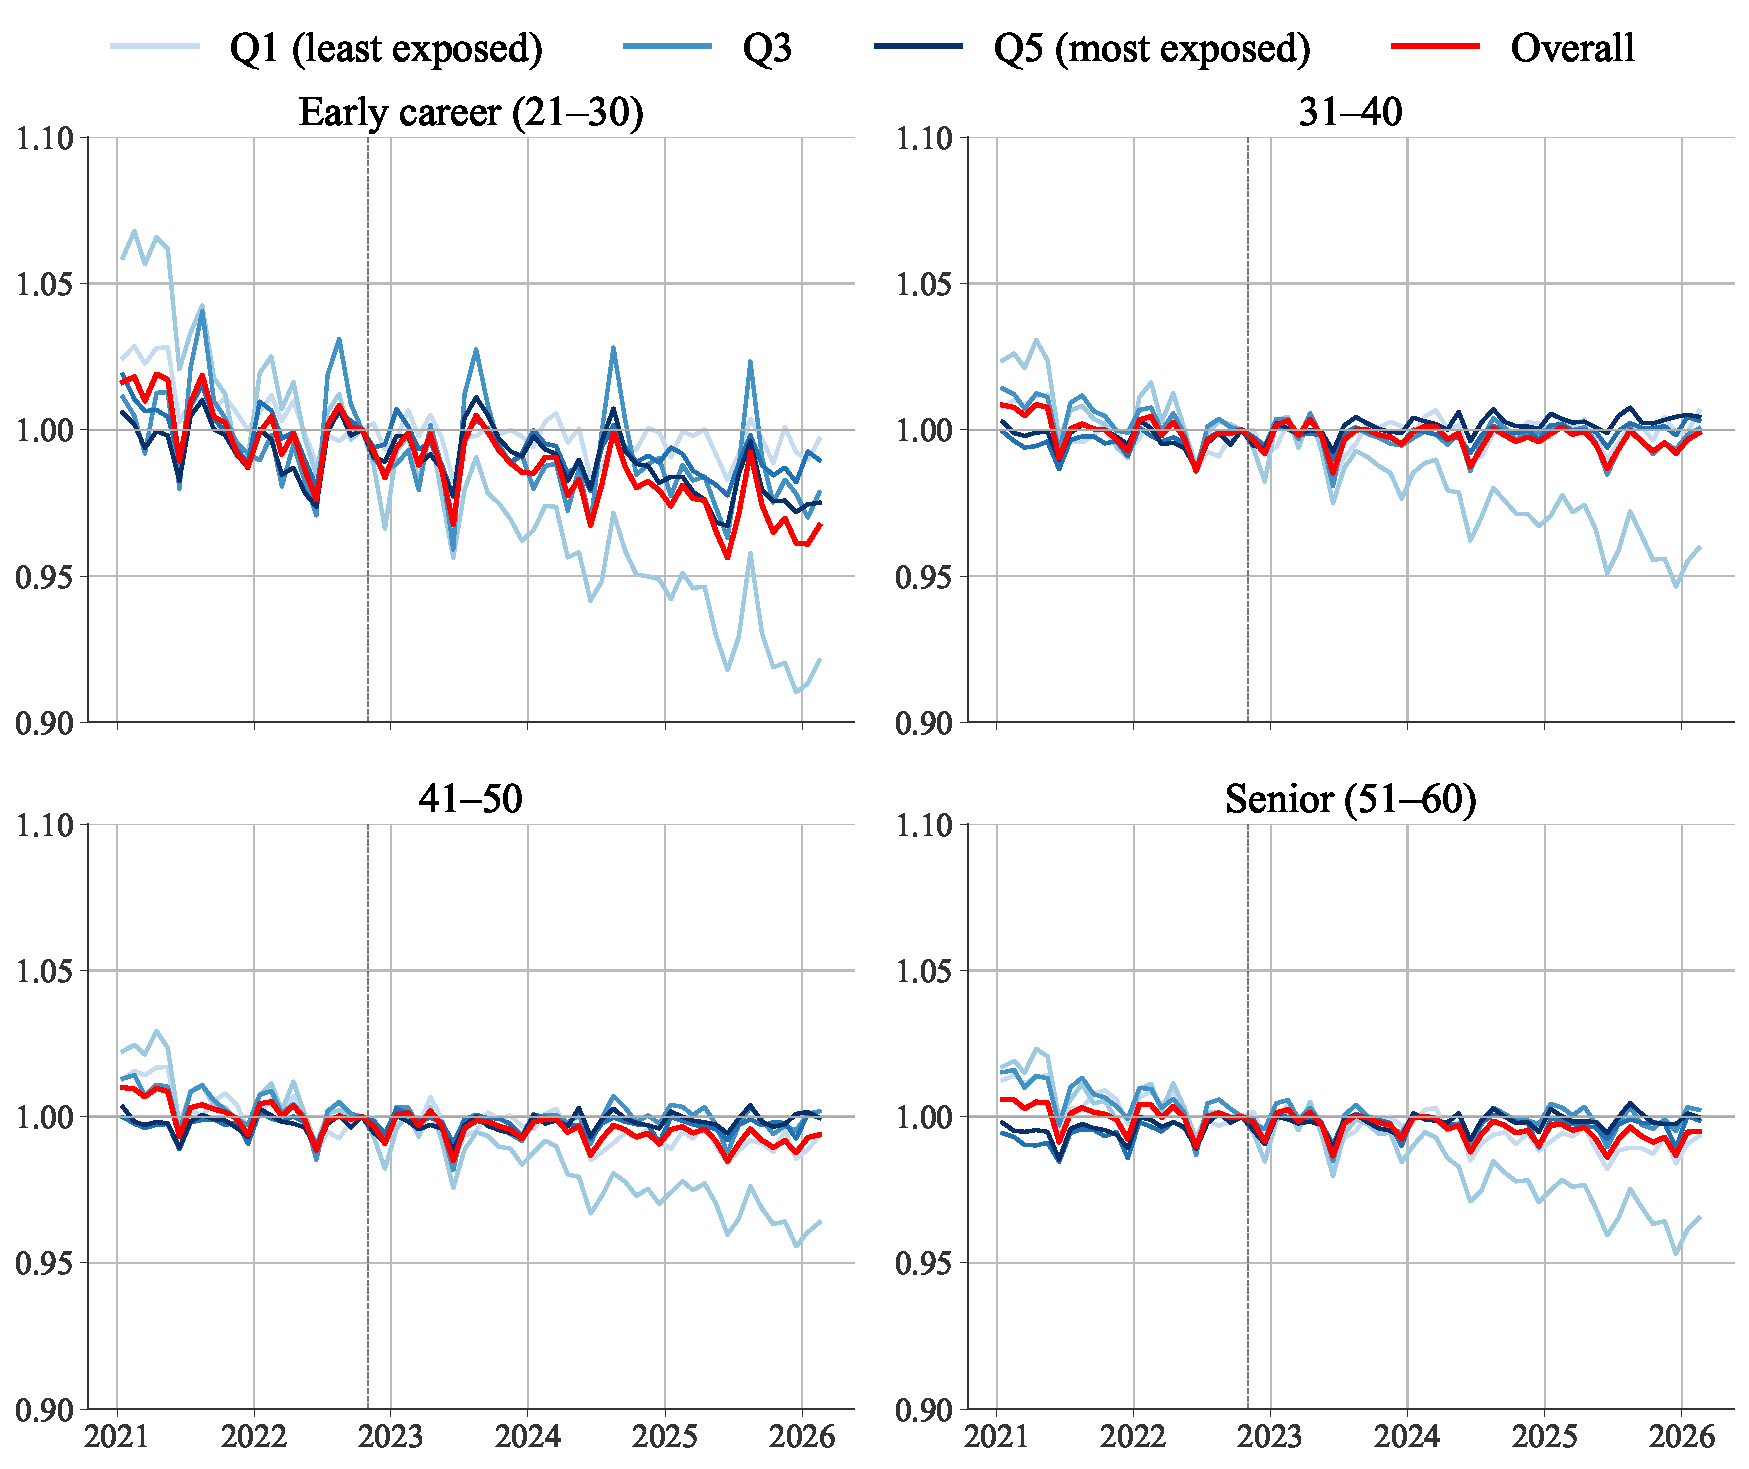
\includegraphics[width=\textwidth]{../analysis/output/figures/figure_stillingspst_decade_private.pdf}
  \caption{Position percentage by AI-exposure quintile and decade age group, private sector.}
  \label{fig:stillingspst_by_quintile}
  \begin{minipage}{\textwidth}\footnotesize\textit{Notes:} Mean contracted position percentage, indexed to October 2022 = 1. Occupations are ranked by the Eloundou et al.\ exposure score.\end{minipage}
\end{figure}

\begin{figure}[htbp]
  \centering
  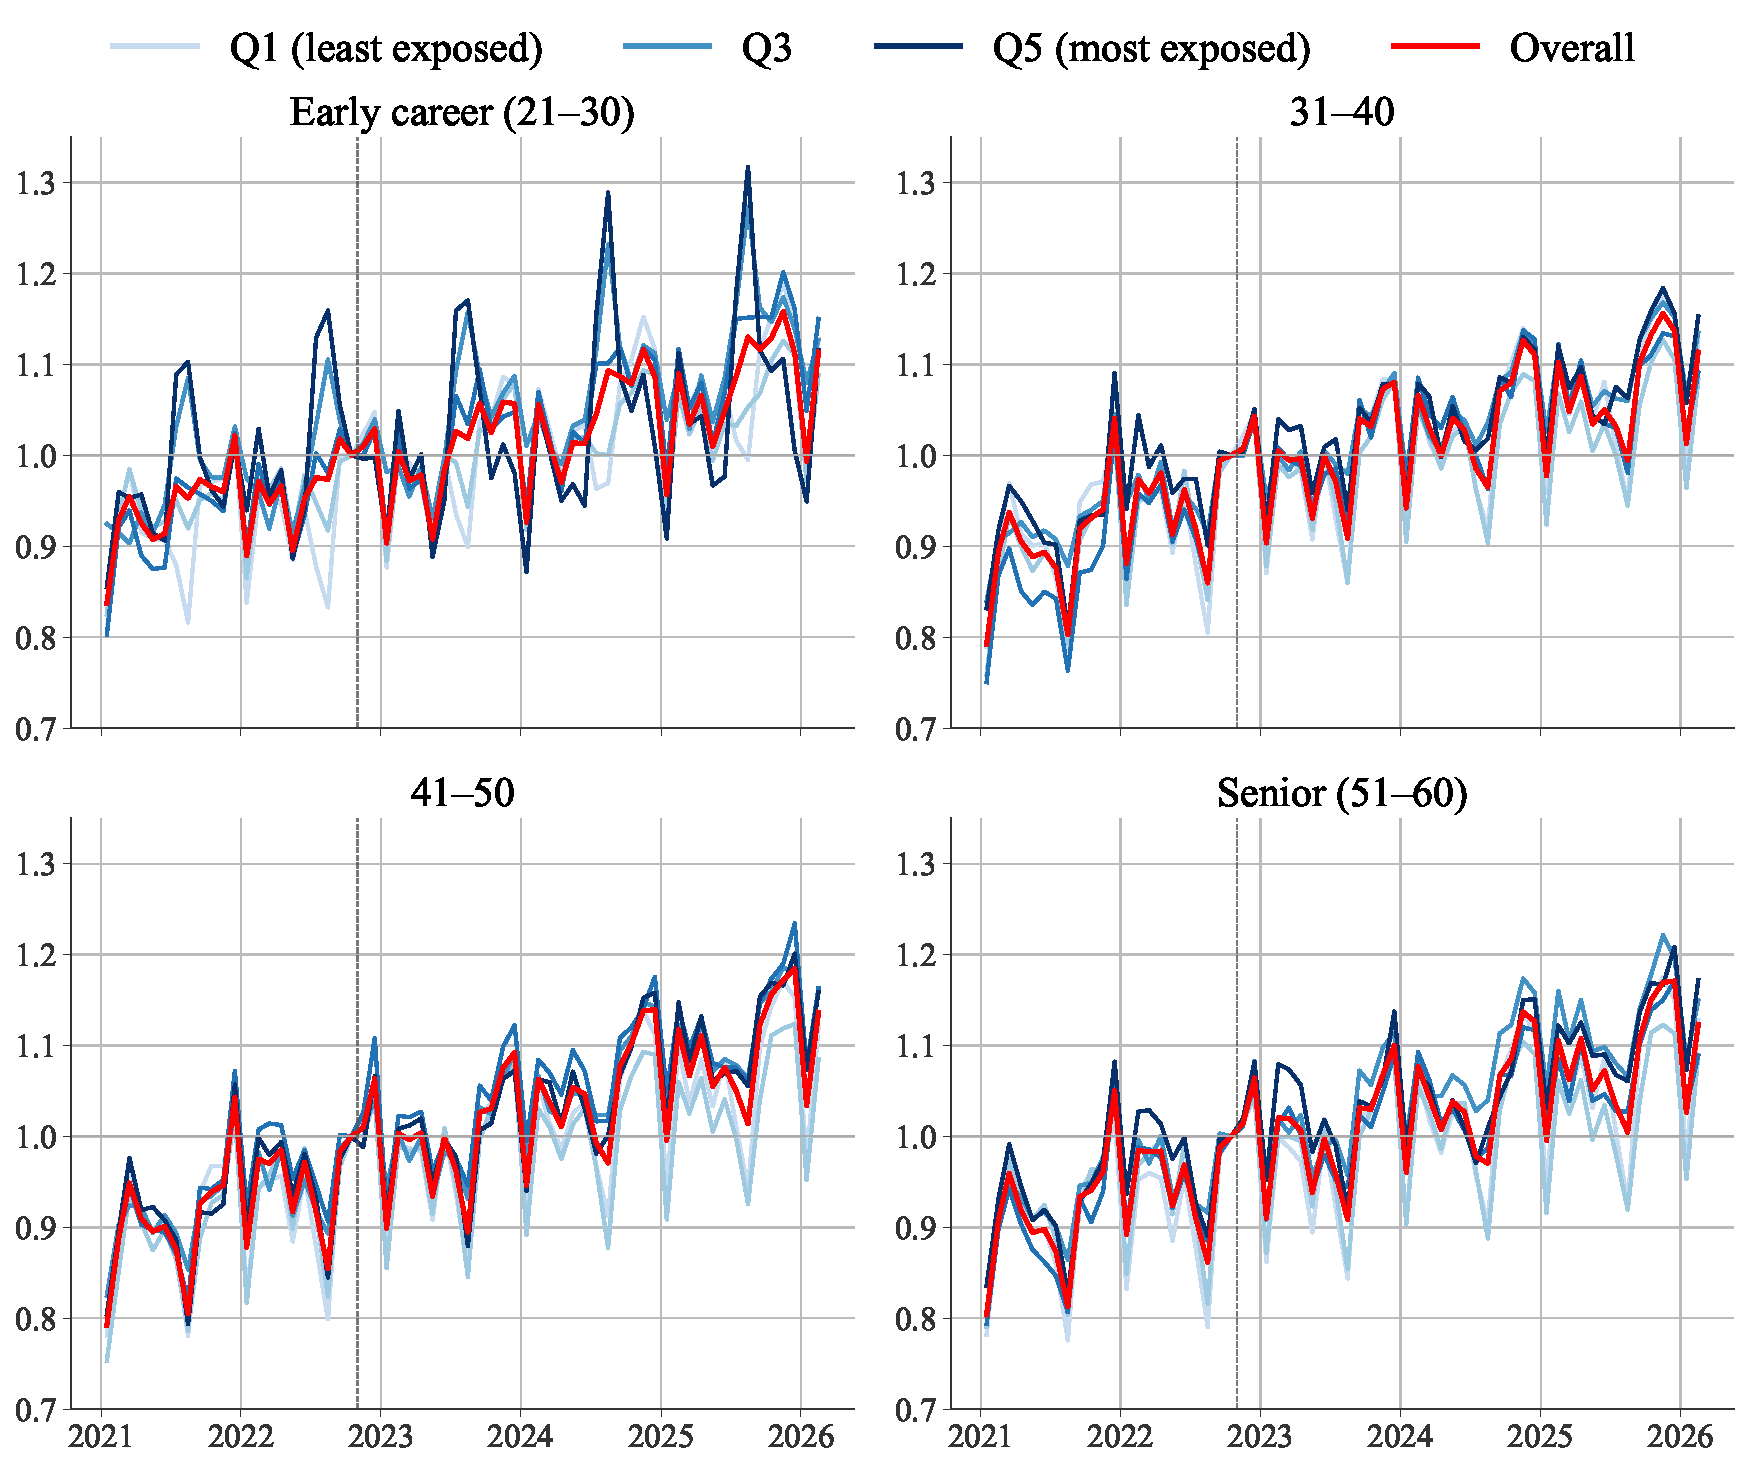
\includegraphics[width=\textwidth]{../analysis/output/figures/figure_timelonn_decade_private.pdf}
  \caption{Hourly wage by AI-exposure quintile and decade age group, private sector.}
  \label{fig:timelonn_by_quintile}
  \begin{minipage}{\textwidth}\footnotesize\textit{Notes:} Mean hourly wage, indexed to October 2022 = 1. Occupations are ranked by the Eloundou et al.\ exposure score.\end{minipage}
\end{figure}

\begin{figure}[htbp]
  \centering
  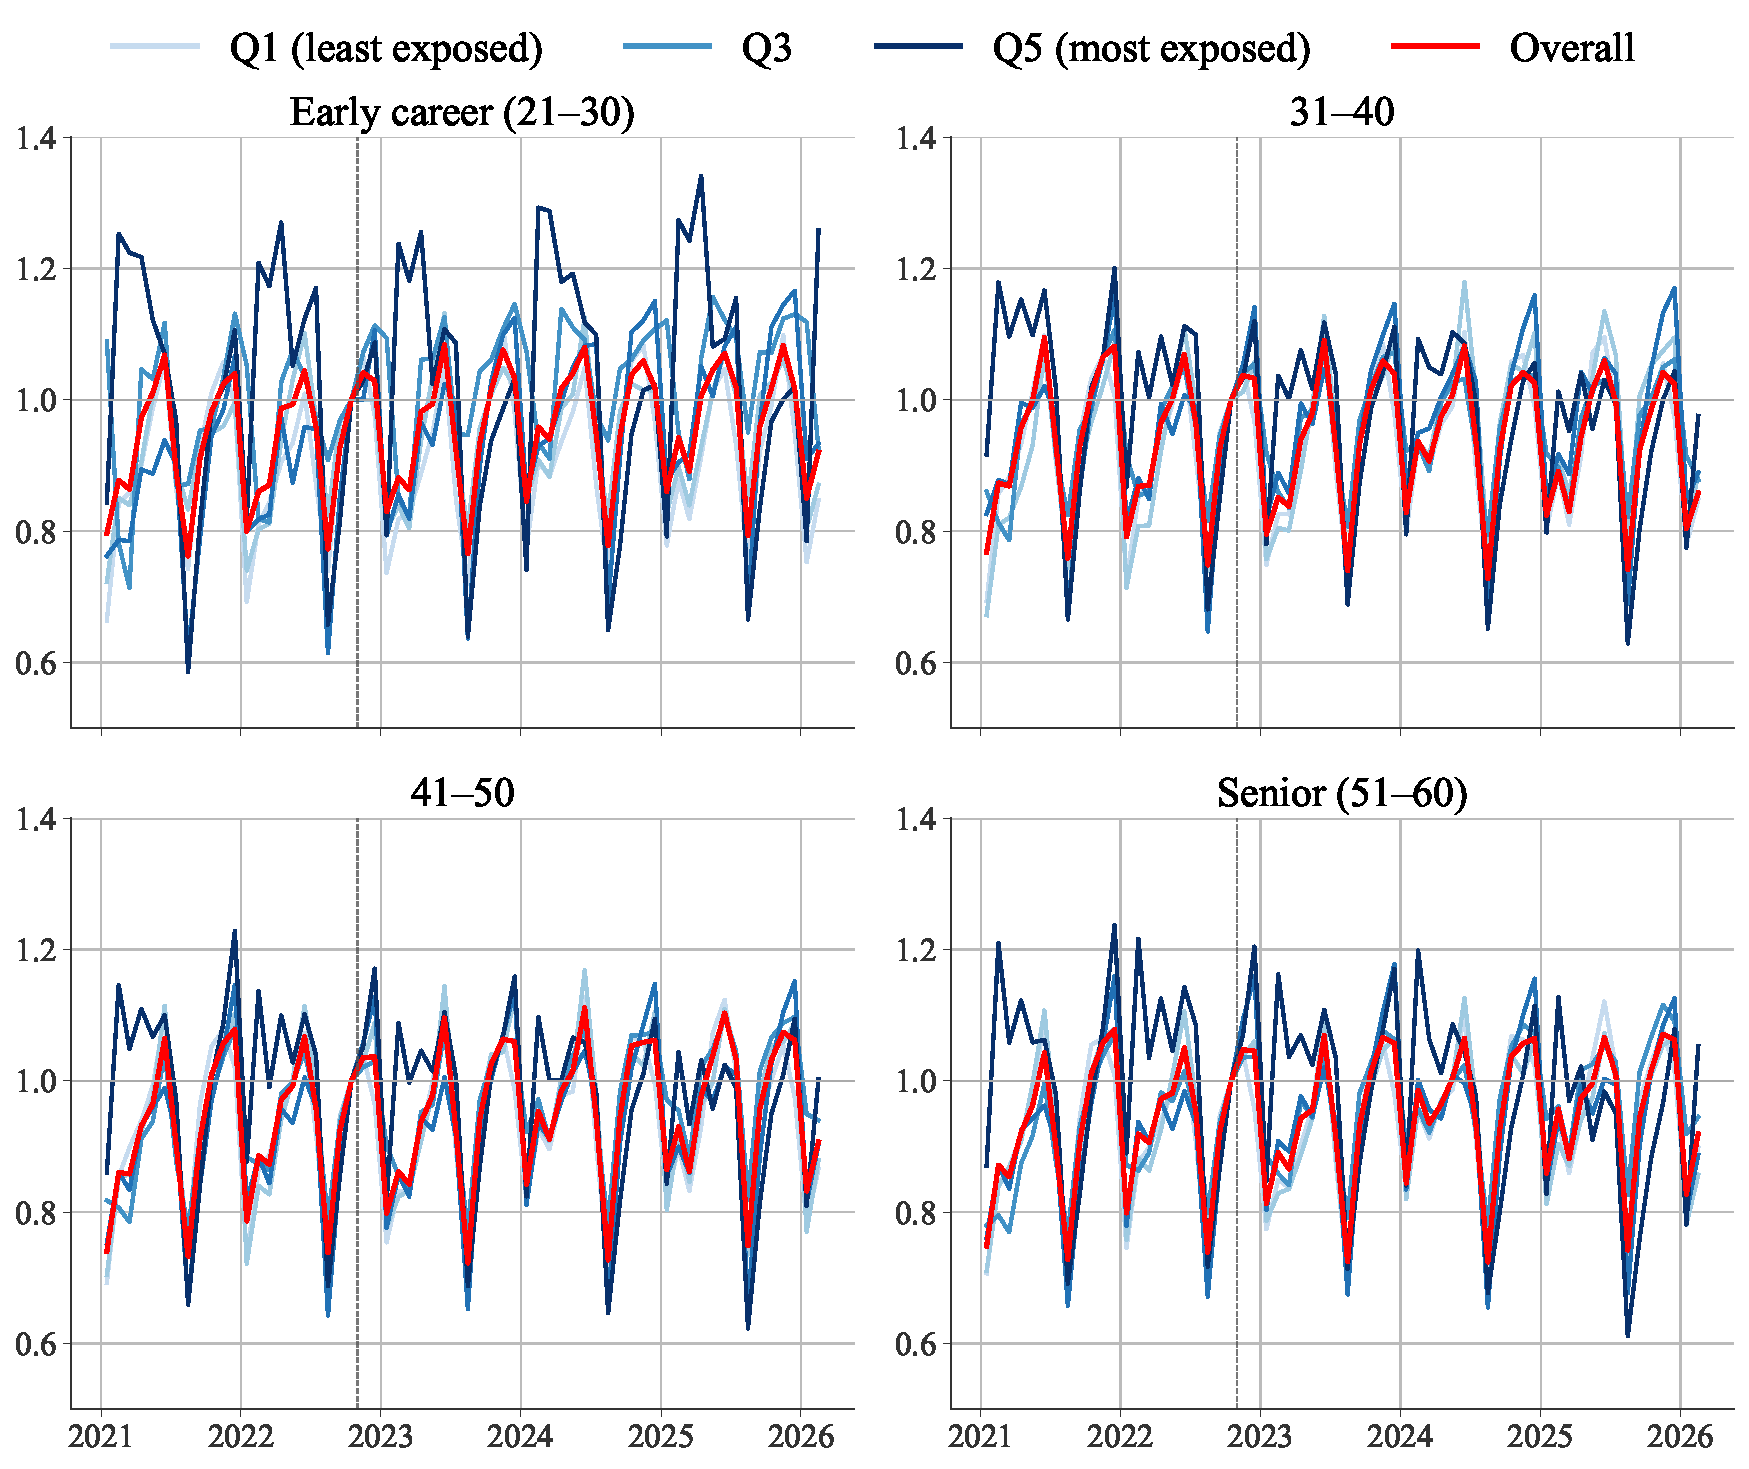
\includegraphics[width=\textwidth]{../analysis/output/figures/figure_overtid_timer_decade_private.pdf}
  \caption{Overtime hours by AI-exposure quintile and decade age group, private sector.}
  \label{fig:overtid_by_quintile}
  \begin{minipage}{\textwidth}\footnotesize\textit{Notes:} Mean overtime hours, indexed to October 2022 = 1. Occupations are ranked by the Eloundou et al.\ exposure score.\end{minipage}
\end{figure}

\begin{figure}[htbp]
  \centering
  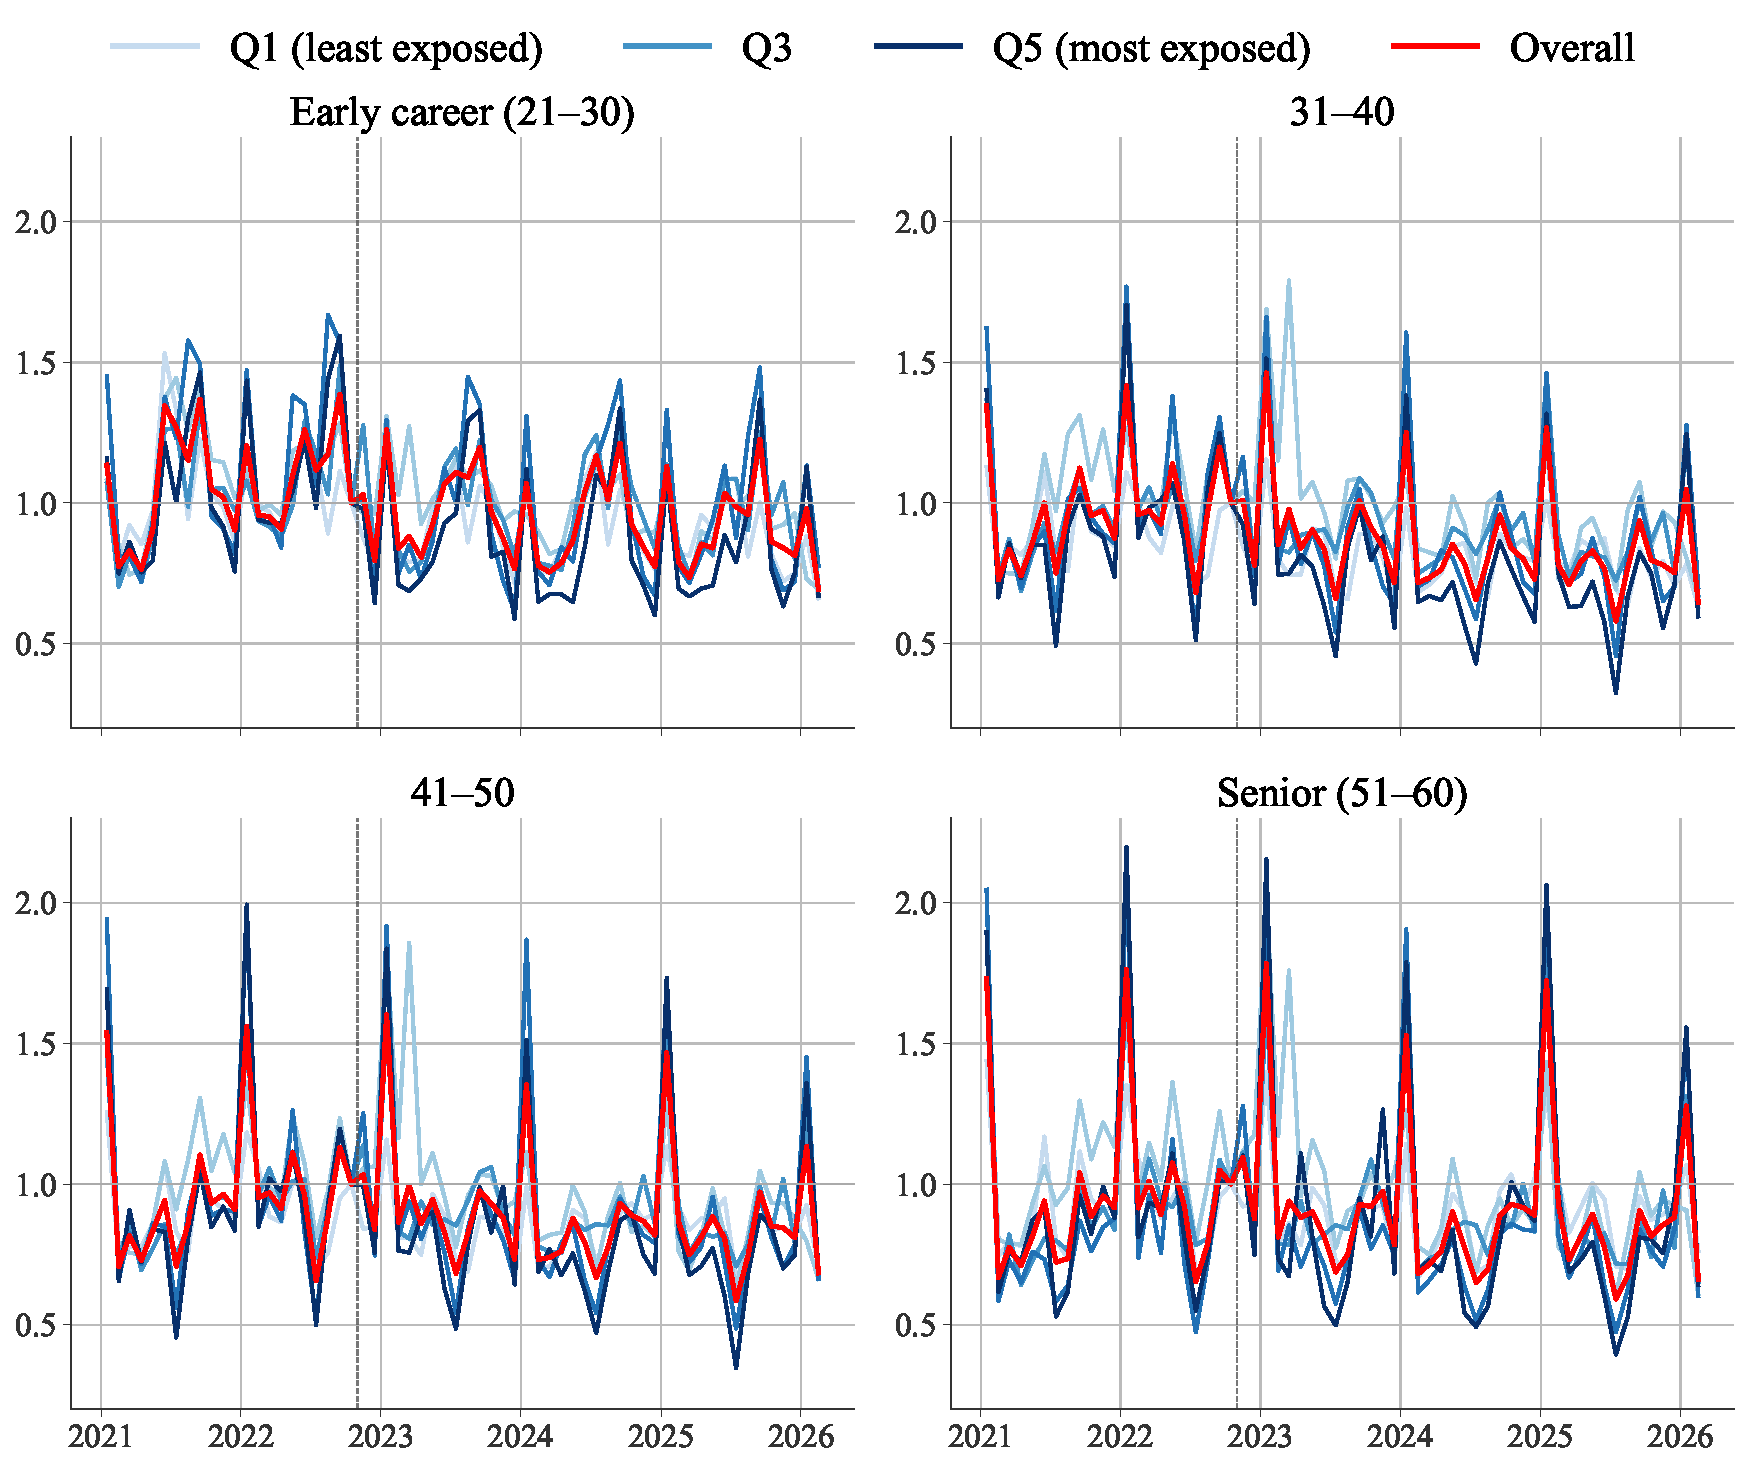
\includegraphics[width=\textwidth]{../analysis/output/figures/figure_ny_jobb_decade_private.pdf}
  \caption{New-hire share by AI-exposure quintile and decade age group, private sector.}
  \label{fig:nyjobb_by_quintile}
  \begin{minipage}{\textwidth}\footnotesize\textit{Notes:} Mean new-hire share, indexed to October 2022 = 1. Occupations are ranked by the Eloundou et al.\ exposure score.\end{minipage}
\end{figure}

\begin{figure}[htbp]
  \centering
  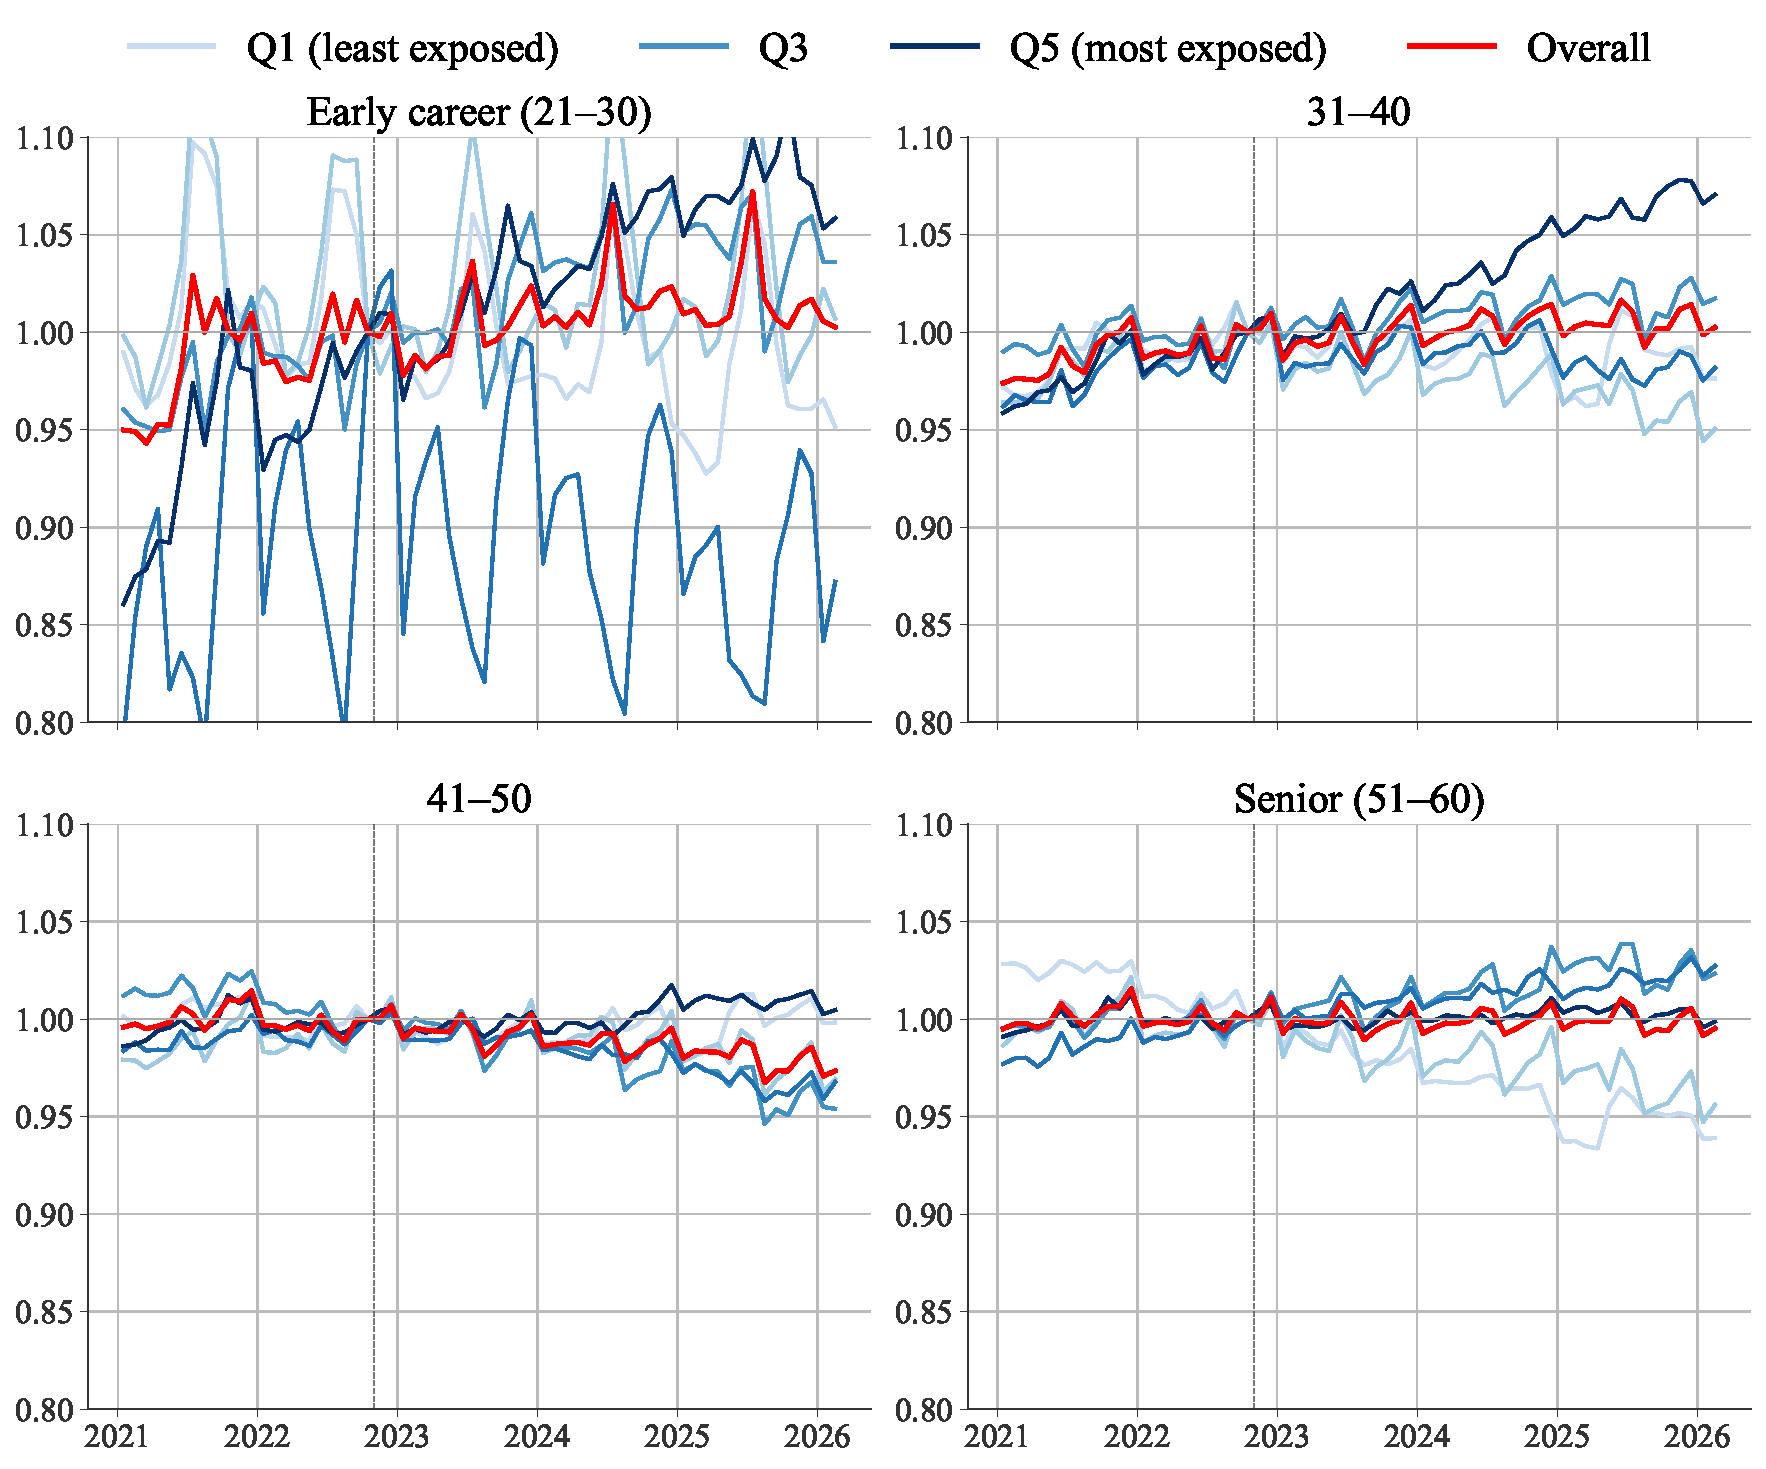
\includegraphics[width=\textwidth]{../analysis/output/figures/figure_emp_decade_public.pdf}
  \caption{Employment by AI-exposure quintile and decade age group, public sector.}
  \label{fig:emp_public}
  \begin{minipage}{\textwidth}\footnotesize\textit{Notes:} Public-sector employment per capita, indexed to October 2022 = 1. Occupations are ranked by the Eloundou et al.\ exposure score. Q1 (lightest) = least exposed; Q5 (darkest) = most exposed. Red line = overall age-group trend. Vertical dashed line marks the November 2022 ChatGPT release.\end{minipage}
\end{figure}

